\section{Infrastructure and Workflow}\label{sec:infrastructure}

Now that we have established our tools requirements, in this section,
we will describe the implementation of our workflow and the minimal infrastructure required to sustend it.

In figure~\ref{fig:project-infra}, we describe our infrastructure that can be first deployed on a local kubernetes single node cluster
with independent DataOps and MLOps pipelines develop by potentially different people with different roles.

\begin{figure}[!htbp]
    \centering
    \caption{Proposed MLOps kubernetes infrastructure using GitOps principles}
    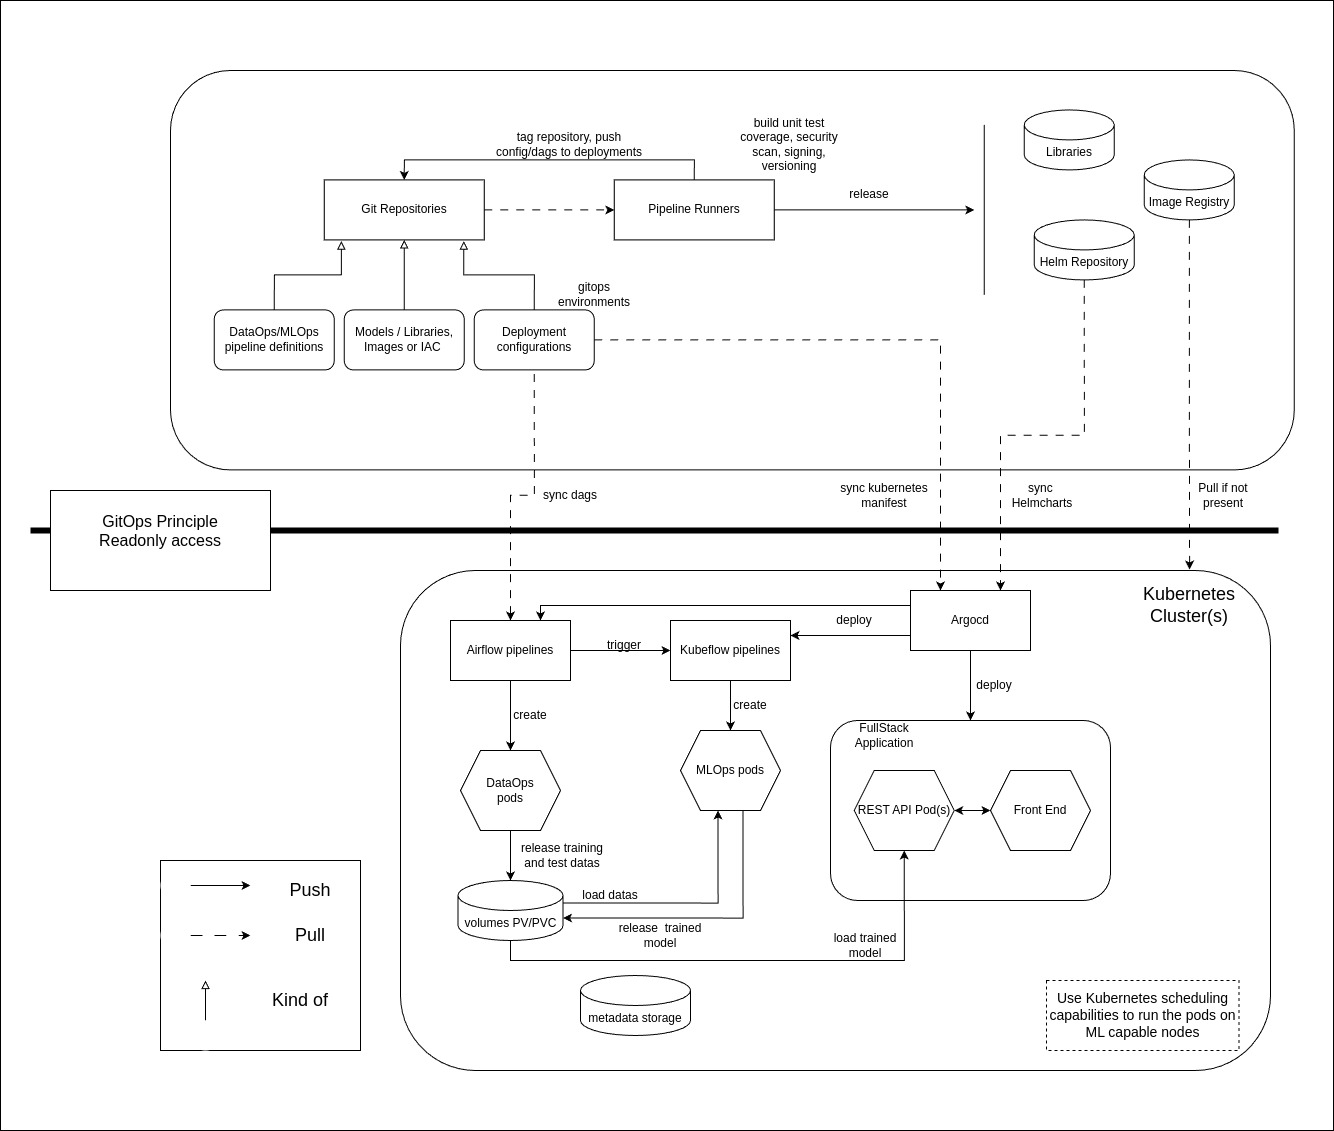
\includegraphics[scale=0.35]{images/project/mthmlops-infra}
    \label{fig:project-infra}
\end{figure}

By using airflow pipelines as general pipelines to trigger our kubeflow pipelines, we can easily gain in maturity towards
more automation by combining the DataOps pipelines and MLOps pipelines together when they are mature enough.

This way we enable kubeflow features for our model developers within a more general purpose environment.

By using the recent git-sync capabilities of Airflow we can synchronise our dags directly with airflow and
even trigger them automatically in a later stage towards automation.

Notably our infrastructure shows the GitOps pull based strategy.
Only the GitHub actions runners do pushes to other git repositories or other
storage like HelmChart repository, images repository any library repository.

We will now further describe the component of our workflow.

\subsection{General workflow}\label{subsec:general-development-workflow}
As previously outlined in our state-of-the-art review, the primary triggers for initiating our workflow are either
the emergence of a new development need or the availability of new data.
Beyond the initial phase—during which the project is discussed and defined in collaboration with business stakeholders.
The motivation for further development or model retraining typically arises from the system's monitoring and feedback loops.

Within our GitOps-based MLOps workflow, any change whether in code or configuration must be committed to the appropriate Git repository.
Each push to the repository triggers a DevOps pipeline, which culminate in updating configuration files in a dedicated configuration repository.
This repository is continuously monitored and synchronised by ArgoCD or Airflow, which applies the changes to the cluster and initiates the DataOps pipeline
or integration tests.
Upon successful completion of this stage, the MLOps pipeline is triggered.
If the newly trained model passes validation criteria, it is released to a model repository.
In accordance with GitOps principles, the deployment involves updating configuration files in a separate Git repository,
enabling ArgoCD to automatically deploy the new model version to the production environment thus closing the automation loop
as shown in figure~\ref{fig:general-workflow}.

\begin{figure}[!htbp]
    \centering
    \caption{General Workflow}
    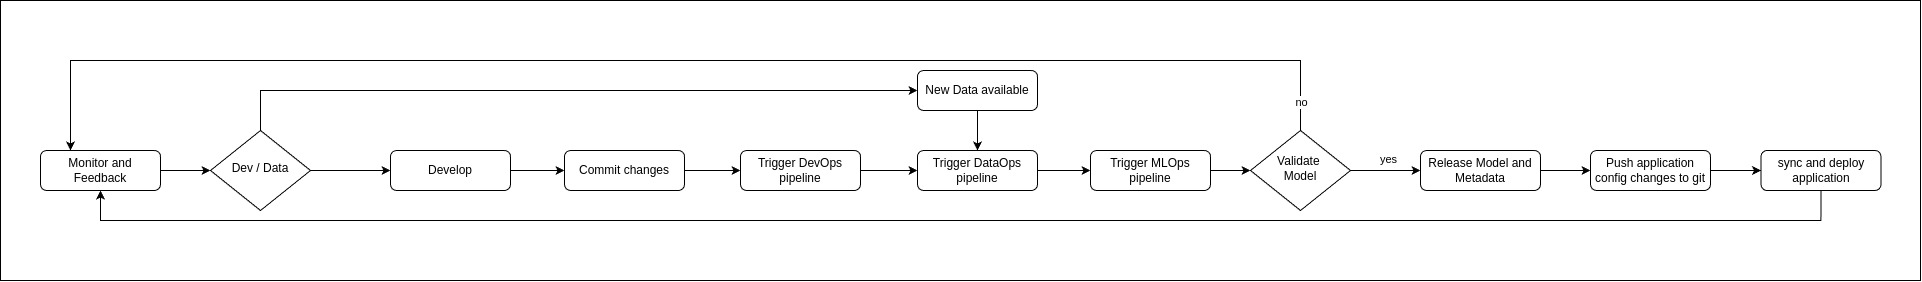
\includegraphics[width=\linewidth]{images/project/general_workflow}
    \label{fig:general-workflow}
\end{figure}

\subsection{Git Repositories}\label{subsec:git-repositories}
As we said, we use Git Repositories for version control and triggering our DevOps pipelines.

Within our infrastructure, we consider 4 types of Git Repositories:

\begin{itemize}
    \item Code Repositories that holds code for models, libraries, docker images and infrastructure as code using Helm.
    \item MLOps and DataOps Pipelines Repositories.
    In our infrastructure those repositories holds the definition of our Airflow DAGs.
    In the first iteration those repositories can also hold images for.


    \item Deployment/Configuration repositories.
    Those repositories are used to hold configuration for the deployed applications and Airflow dags.
    We use ArgoCD GitOps implementation to synchronise changes to those repositories.
    Airflow git/sync feature allows us to synchronise our dags with
    Change in those repositories can be automated by the pipeline runners.
    Depending on your team and organization those repositories can be separated into multiple repositories (per team, per domain, per environment (dev,test,staging,prod))
    For the Dev environment we allow developers to push from their code repositories within those repositories.
    For the production environment we use a pipeline to pull the configuration from the staging environment.
    We called this promote our configuration to a new environment.
    In case of full automation the pulling/promotion can be trigger automatically by ArgoCD sending webhooks on any test results desired.
    \item CI/CD pipelines templates
    In those we define workflows that can be used in any repository to be used by the developers.
    It includes building image workflows, versioning with tags on repositories, pushing new configurations into deployments repositories.
    By defining them in a separate repository it allows us to version them and make it easy for developers to choose a workflow.
    Each workflow is closely tight to the structure of the repository, so we defined one per type of repositories.
\end{itemize}

Following GitOps principle those are the source of truth for all our code and configurations, for the infrastructure, the pipelines, the model and the software development.
We adopt a consistent structure (figure~\ref{fig:sidebyside}) for both our DataOps and MLOps pipeline repositories, incorporating a config.yml file that mirrors the organizational pattern of our Helm chart repositories.
In both cases, an images directory is used to define containerized steps for the pipelines and for deployment configurations within the Helm charts.
This consistency permit to reuse our Devops pipelines templates.

\begin{figure}[h!]
    \centering
    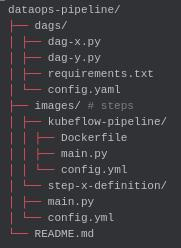
\includegraphics[scale=0.35]{images/project/git-repo-dataops}
    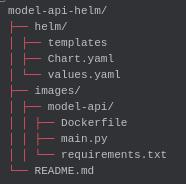
\includegraphics[scale=0.35]{images/project/git-repo-helm}
    \caption{Consistent structure within repositories}
    \label{fig:sidebyside}
\end{figure}


\subsubsection{General Rules for Managing Git Repositories}
We follow the GitHub flow with adaptations to fit our workflow.
However, it can be adjusted as needed.

\begin{itemize}
    \item A Pull Request is required for merging into the \texttt{main} branch, including a pipeline run and team review.
    \item Follow GitHub flow, using \texttt{feature/} and \texttt{hotfix/} branches for development.
    \item Approvals are required for deploying to environment-specific repositories.
    \item The \texttt{main} branch is deployed to the production environment or released into production Docker/Helm repositories.
    \item Other branches are deployed sequentially to all environments, passing tests and approval gates before merging to main.
\end{itemize}

\subsection{GitOps}
With a Helm-based installation pipeline, the runner requires write access to push applications directly to Kubernetes.
By adopting ArgoCD and a GitOps approach, we eliminate this requirement by pulling changes directly from GitHub.
This enables all operations to be managed within GitHub.
However, it necessitates properly configured permissions in GitHub to prevent potential security breaches.

Airflow also integrate a Git/Sync feature that allows us to load and trigger the DAGs within Airflow.

\subsection{DataOps pipelines}
DataOps pipelines are defined as Airflow DAGs that will, with the KubernetesExecutor functionality of Airflow,
create pods for every step defined in the pipeline.
They can be connected to an observability stack like OpenSearch to analyse and store the data.
This can be used as Monitoring tools for all our infrastructure too.

\begin{figure}[!htbp]
    \centering
    \caption{Example of a DataOps pipeline define within Airflow}
    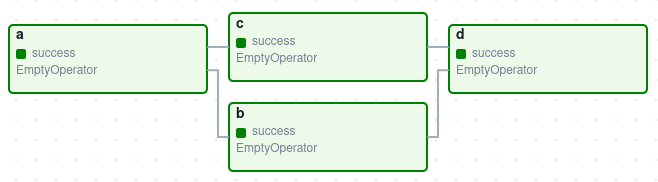
\includegraphics[scale=0.5]{images/project/data-ops-airflow-dag}
    \label{fig:project-data-ops-airflow-dag}
\end{figure}

\subsection{MLOps pipelines}
Kubeflow allows us to deploy all the required steps within our MLOps pipeline by creating pods in the required namespace within our Kubernetes cluster.
A lot like Airflow would.
We use Kubeflow to allow our ML engineer to use other features like model and metadata storage.
Other features from the Kubeflow ecosystem could be added at any time if necessary.

\begin{figure}[!htbp]
    \centering
    \caption{Example of a MLOps pipeline define within Airflow}
    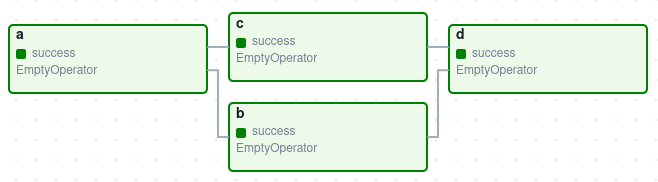
\includegraphics[scale=0.5]{images/project/data-ops-airflow-dag}
    \label{fig:project-ml-ops-airflow-dag}
\end{figure}

